\section{Marco Teorico } 
\begin{flushleft}
\begin{itemize}
\textbf{}\\
El Modelo Relacional es un modelo de datos basado en la lógica de predicado y en la teoría de conjuntos para  la  gestión  de  una  base  de  datos.  Siguiendo  este  modelo  se  puede  construir  una  base  de  datos relacional  que no  es  más  que  un  conjunto  de  una  o  más  tablas  estructuradas  en  registros  (filas)  y campos  (columnas),  que  se  vinculan  entre  sí  por  un  campo  en  común.  Sin  embargo,  en  el  Modelo Orientado a Objetos en una única entidad denominada objeto, se combinan las estructuras de datos con sus  comportamientos.  En  este  modelo  se  destacan  conceptos  básicos  tales  como  objetos,  clases  y herencia.

\textbf{}\\
La gran mayoría de los lenguajes de programación como java o C, tienen un modelo de manejo de datos basado en leer, escribir o modificar registros de uno en uno. Por ello, cuando se  invoca el lenguaje de consulta   SQL   (Standard   Query   Language)   desde   un   lenguaje   de   programación   es   necesario   un mecanismo de vinculación que permita recorrer las filas de una consulta a la base de datos y acceder de forma individual a cada una de ellas

\textbf{}\\
Además en el modelorelacional no se puede modelar la herencia que aparece en el modelo orientado a objetos  y  existen  también  desajustes  en  los  tipos  de  datos,  ya  que  los  tipos  y  denotaciones  de  tipos asumidos por las consultas y lenguajes de programación difieren. Esto concierne a tipos atómicos como integer,  real,  boolean,  etc.  La  representación  de  tipos  atómicos  en  lenguajes  de  programación  y  en bases de datos pueden ser significativamente diferentes, incluso si los tipos son denotados por la misma palabra  reservada,  ej.: integer.  Esto  ocurre  también  con  tipos  complejos  como  las  tablas,  un  tipo  de datos básico en SQL ausente en los lenguajes de programación. 

\textbf{}\\
Para  atenuar  los  efectos  del  desajuste  por  impedancia  entre  ambos  modelos  existen  varias  técnicas  y prácticas  como  los  Objetos  de  Acceso  a  Datos  (Data  Acces  Objects  o  DAOs),  marcos  de  trabajo  de persistencia  (Persistence  Frameworks),  mapeadores Objeto/Relacionales  (Object/Relational  Mappers  u ORM), consultas nativas (Native Queries), lenguajes integrados como PL-SQL de Oracle y T-SQL de SQL Server; mediadores, repositorios virtuales y bases de datos orientadas a objetos

\textbf{}\\
Mapeo Objeto/Relacional

\textbf{}\\
El  mapeo  objeto-relacional  es  una  técnica  de  programación para  convertir  datos  del  sistema  de  tipos utilizado  en  un  lenguaje  de  programación  orientado  a  objetos  al  utilizado  en  una  base  de  datos relacional. En la práctica esto crea una base de datos virtual orientada a objetos sobre la base de datos relacional. Esto posibilita el uso de las características propias de la orientación a objetos (esencialmente la herencia y el polimorfismo).

\textbf{}\\
Las  bases  de  datos  relacionales  solo  permiten  guardar  tipos  de  datos  primitivos  (enteros,  cadenas  de texto, etc.) por lo que no se pueden guardar de forma directa los objetos de la aplicación en las tablas, sino que estos se deben de convertir antes en registros, que por lo general afectan a varias tablas. En el momento  de  volver  a  recuperar  los  datos,  hay  que  hacer  el  proceso  contrario,  se  deben  convertir  los registros  en  objetos.  Es  entonces  cuando  ORM  cobra  importancia,  ya  que  se  encarga  de  forma automática  de  convertir  los  objetos  en  registros  y  viceversa,  simulando  así  tener  una  base  de  datos orientada a objetos.

\begin{center}
    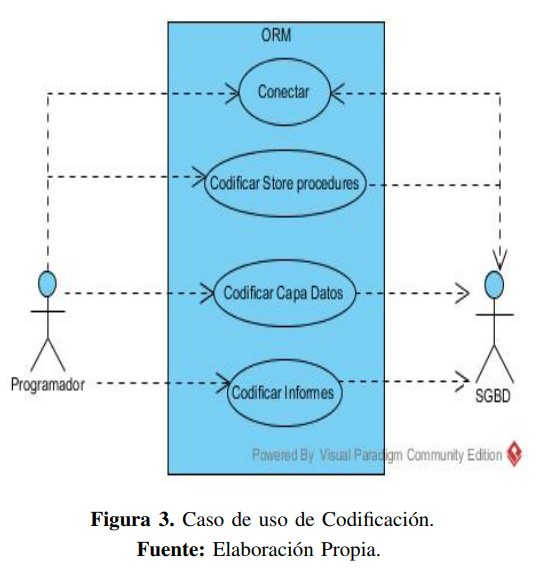
\includegraphics[width=12cm]{./Imagenes/ORM}
 \end{center}
\begin{center}
    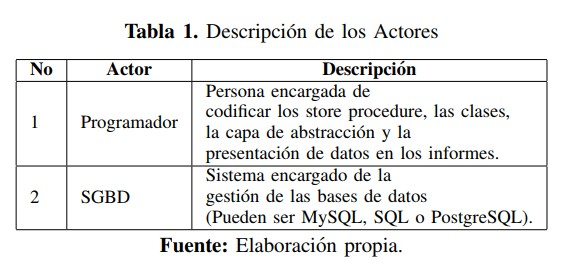
\includegraphics[width=12cm]{./Imagenes/ACTORES}
 \end{center}
\end{itemize} 


\end{flushleft}